\documentclass[tikz,border=5pt]{standalone}
\usepackage[UTF8]{ctex}
\usepackage{amsmath}
\usetikzlibrary{arrows.meta,calc}
\definecolor{blue}{RGB}{45,98,142}
\definecolor{red}{RGB}{175,67,51}
\definecolor{green}{RGB}{60,117,87}
\newcommand{\boxedges}{
\draw[gray,dashed](0,0,0)--(0,1,0)--(1,1,0);
\draw[gray,dashed](0,1,0)--(0,1,1);
\draw[thick](0,0,0)--(1,0,0)--(1,1,0)--(1,1,1)--(0,1,1)--(0,0,1)--cycle;
\draw[thick](1,0,0)--(1,0,1)--(0,0,1);
\draw[thick](1,0,1)--(1,1,1);
}
\begin{document}
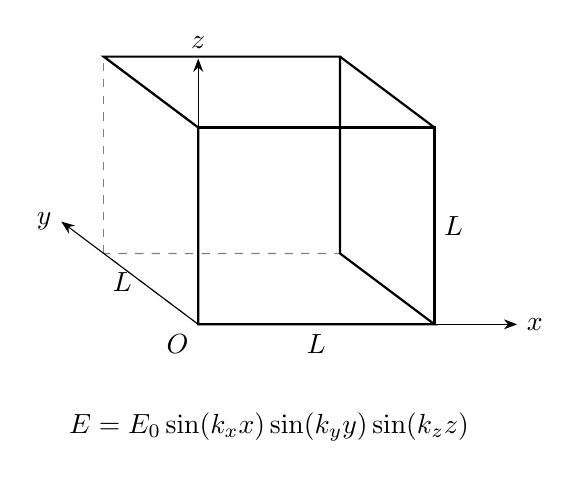
\begin{tikzpicture}[x={(3cm,0cm)},y={(-1.2cm,.9cm)},z={(0cm,2.5cm)}]
\boxedges
\draw[-{Stealth}](0,0,0)--(1.35,0,0)node[right]{$x$};
\draw[-{Stealth}](0,0,0)--(0,1.45,0)node[left]{$y$};
\draw[-{Stealth}](0,0,0)--(0,0,1.35)node[above]{$z$};
\node[below left]at(0,0,0){$O$};
\node[below]at(.5,0,0){$L$};\node[left]at(0,.6,0){$L$};\node[right]at(1,0,.5){$L$};
\node at(.5,.5,-.7){$E=E_0\sin(k_xx)\sin(k_yy)\sin(k_zz)$};
\end{tikzpicture}
\begin{tikzpicture}[x={(3cm,0cm)},y={(-1.2cm,.9cm)},z={(0cm,2.5cm)}]
\boxedges
\draw[red,very thick](0,1,1)--(1,1,1);
\draw[blue,fill=blue!8,fill opacity=.3](0,0,1)--(1,0,1)--(1,1,1)--(0,1,1)--cycle;
\node[red,above]at(.5,1,1){棱：$y=z=L$};
\node[blue,right]at(1.1,0,.9){面：$z=L$};
\node[align=center]at(.5,.4,-.75){棱上：$\sin(k_yL)\sin(k_zL)=0$\\面上非零模：须 $\sin(k_zL)=0$};
\end{tikzpicture}
\begin{tikzpicture}[x={(1.05cm,0cm)},y={(-.5cm,.42cm)},z={(0cm,.85cm)}]
\foreach \x in{-1,0,1}{\foreach \y in{-1,0,1}{\foreach \z in{-1,0,1}{\fill[blue](\x,\y,\z)circle(1.6pt);}}}
\draw[-{Stealth}](-1.5,0,0)--(2,0,0)node[right]{$k_x$};
\draw[-{Stealth}](0,-1.5,0)--(0,2,0)node[left]{$k_y$};
\draw[-{Stealth}](0,0,-1.5)--(0,0,2)node[above]{$k_z$};
\draw[red,thick](0,0,0)--(1,0,0)--(1,1,0)--(0,1,0)--cycle;
\draw[red,thick](0,0,1)--(1,0,1)--(1,1,1)--(0,1,1)--cycle;
\foreach \x/\y in{0/0,1/0,1/1,0/1}{\draw[red](\x,\y,0)--(\x,\y,1);}
\draw[gray,<->](0,-.8,-1.6)--node[below]{$\pi/L$}(1,-.8,-1.6);
\node at(.2,0,-2.8){单格体积 $(\pi/L)^3$；包含正负标签};
\end{tikzpicture}
\begin{tikzpicture}
\draw[fill=blue!5](0,0)circle(2);
\draw[red,fill=red!8](0,0)circle(1.45);\draw[fill=blue!5](0,0)circle(1.3);
\draw[gray,dashed](0,0)ellipse(2 and .55);
\draw[gray](0,0)ellipse(1.45 and .4);\draw[gray](0,0)ellipse(1.3 and .36);
\draw[-{Stealth}](-2.4,0)--(2.7,0)node[right]{$k_x$};
\draw[-{Stealth}](0,-2.4)--(0,2.6)node[above]{$k_z$};
\draw[-{Stealth}](1.8,-1.1)--(-2,1.3)node[left]{$k_y$};
\draw[blue,-{Stealth}](0,0)--(45:2)node[above right]{$k_{\max}$};
\draw[red,<->](25:1.3)--(25:1.45);
\node[red,right]at(1.8,.85){$dk$};
\node at(0,-3.1){薄壳：$dN=(V/\pi^3)4\pi k^2dk$};
\node at(0,-3.7){每态能量 $\hbar ck$，覆盖八个卦限};
\end{tikzpicture}
\end{document}
